\documentclass[12pt]{article}
%Fall 2022
% Some basic packages
\usepackage{standalone}[subpreambles=true]
\usepackage[utf8]{inputenc}
\usepackage[T1]{fontenc}
\usepackage{textcomp}
\usepackage[english]{babel}
\usepackage{url}
\usepackage{graphicx}
%\usepackage{quiver}
\usepackage{float}
\usepackage{enumitem}
\usepackage{lmodern}
\usepackage{comment}
\usepackage{hyperref}
\usepackage[usenames,svgnames,dvipsnames]{xcolor}
\usepackage[margin=1in]{geometry}
\usepackage{pdfpages}

\pdfminorversion=7

% Don't indent paragraphs, leave some space between them
\usepackage{parskip}

% Hide page number when page is empty
\usepackage{emptypage}
\usepackage{subcaption}
\usepackage{multicol}
\usepackage[b]{esvect}

% Math stuff
\usepackage{amsmath, amsfonts, mathtools, amsthm, amssymb}
\usepackage{bbm}
\usepackage{stmaryrd}
\allowdisplaybreaks

% Fancy script capitals
\usepackage{mathrsfs}
\usepackage{cancel}
% Bold math
\usepackage{bm}
% Some shortcuts
\newcommand{\rr}{\ensuremath{\mathbb{R}}}
\newcommand{\zz}{\ensuremath{\mathbb{Z}}}
\newcommand{\qq}{\ensuremath{\mathbb{Q}}}
\newcommand{\nn}{\ensuremath{\mathbb{N}}}
\newcommand{\ff}{\ensuremath{\mathbb{F}}}
\newcommand{\cc}{\ensuremath{\mathbb{C}}}
\newcommand{\ee}{\ensuremath{\mathbb{E}}}
\newcommand{\hh}{\ensuremath{\mathbb{H}}}
\renewcommand\O{\ensuremath{\emptyset}}
\newcommand{\norm}[1]{{\left\lVert{#1}\right\rVert}}
\newcommand{\dbracket}[1]{{\left\llbracket{#1}\right\rrbracket}}
\newcommand{\ve}[1]{{\bm{#1}}}
\newcommand\allbold[1]{{\boldmath\textbf{#1}}}
\DeclareMathOperator{\lcm}{lcm}
\DeclareMathOperator{\im}{im}
\DeclareMathOperator{\coim}{coim}
\DeclareMathOperator{\dom}{dom}
\DeclareMathOperator{\tr}{tr}
\DeclareMathOperator{\rank}{rank}
\DeclareMathOperator*{\var}{Var}
\DeclareMathOperator*{\ev}{E}
\DeclareMathOperator{\dg}{deg}
\DeclareMathOperator{\aff}{aff}
\DeclareMathOperator{\conv}{conv}
\DeclareMathOperator{\inte}{int}
\DeclareMathOperator*{\argmin}{argmin}
\DeclareMathOperator*{\argmax}{argmax}
\DeclareMathOperator{\graph}{graph}
\DeclareMathOperator{\sgn}{sgn}
\DeclareMathOperator*{\Rep}{Rep}
\DeclareMathOperator{\Proj}{Proj}
\DeclareMathOperator{\mat}{mat}
\DeclareMathOperator{\diag}{diag}
\DeclareMathOperator{\aut}{Aut}
\DeclareMathOperator{\gal}{Gal}
\DeclareMathOperator{\inn}{Inn}
\DeclareMathOperator{\edm}{End}
\DeclareMathOperator{\Hom}{Hom}
\DeclareMathOperator{\ext}{Ext}
\DeclareMathOperator{\tor}{Tor}
\DeclareMathOperator{\Span}{Span}
\DeclareMathOperator{\Stab}{Stab}
\DeclareMathOperator{\cont}{cont}
\DeclareMathOperator{\Ann}{Ann}
\DeclareMathOperator{\Div}{div}
\DeclareMathOperator{\curl}{curl}
\DeclareMathOperator{\nat}{Nat}
\DeclareMathOperator{\gr}{Gr}
\DeclareMathOperator{\vect}{Vect}
\DeclareMathOperator{\id}{id}
\DeclareMathOperator{\Mod}{Mod}
\DeclareMathOperator{\sign}{sign}
\DeclareMathOperator{\Surf}{Surf}
\DeclareMathOperator{\fcone}{fcone}
\DeclareMathOperator{\Rot}{Rot}
\DeclareMathOperator{\grad}{grad}
\DeclareMathOperator{\atan2}{atan2}
\DeclareMathOperator{\Ric}{Ric}
\let\vec\relax
\DeclareMathOperator{\vec}{vec}
\let\Re\relax
\DeclareMathOperator{\Re}{Re}
\let\Im\relax
\DeclareMathOperator{\Im}{Im}
% Put x \to \infty below \lim
\let\svlim\lim\def\lim{\svlim\limits}

%wide hat
\usepackage{scalerel,stackengine}
\stackMath
\newcommand*\wh[1]{%
\savestack{\tmpbox}{\stretchto{%
  \scaleto{%
    \scalerel*[\widthof{\ensuremath{#1}}]{\kern-.6pt\bigwedge\kern-.6pt}%
    {\rule[-\textheight/2]{1ex}{\textheight}}%WIDTH-LIMITED BIG WEDGE
  }{\textheight}% 
}{0.5ex}}%
\stackon[1pt]{#1}{\tmpbox}%
}
\parskip 1ex

%Make implies and impliedby shorter
\let\implies\Rightarrow
\let\impliedby\Leftarrow
\let\iff\Leftrightarrow
\let\epsilon\varepsilon

% Add \contra symbol to denote contradiction
\usepackage{stmaryrd} % for \lightning
\newcommand\contra{\scalebox{1.5}{$\lightning$}}

% \let\phi\varphi

% Command for short corrections
% Usage: 1+1=\correct{3}{2}

\definecolor{correct}{HTML}{009900}
\newcommand\correct[2]{\ensuremath{\:}{\color{red}{#1}}\ensuremath{\to }{\color{correct}{#2}}\ensuremath{\:}}
\newcommand\green[1]{{\color{correct}{#1}}}

% horizontal rule
\newcommand\hr{
    \noindent\rule[0.5ex]{\linewidth}{0.5pt}
}

% hide parts
\newcommand\hide[1]{}

% si unitx
\usepackage{siunitx}
\sisetup{locale = FR}

%allows pmatrix to stretch
\makeatletter
\renewcommand*\env@matrix[1][\arraystretch]{%
  \edef\arraystretch{#1}%
  \hskip -\arraycolsep
  \let\@ifnextchar\new@ifnextchar
  \array{*\c@MaxMatrixCols c}}
\makeatother

\renewcommand{\arraystretch}{0.8}

\renewcommand{\baselinestretch}{1.5}

\usepackage{graphics}
\usepackage{epstopdf}

\RequirePackage{hyperref}
%%
%% Add support for color in order to color the hyperlinks.
%% 
\hypersetup{
  colorlinks = true,
  urlcolor = blue,
  citecolor = blue
}
%%fakesection Links
\hypersetup{
    colorlinks,
    linkcolor={red!50!black},
    citecolor={green!50!black},
    urlcolor={blue!80!black}
}
%customization of cleveref
\RequirePackage[capitalize,nameinlink]{cleveref}[0.19]

% Per SIAM Style Manual, "section" should be lowercase
\crefname{section}{section}{sections}
\crefname{subsection}{subsection}{subsections}
\Crefname{section}{Section}{Sections}
\Crefname{subsection}{Subsection}{Subsections}

% Per SIAM Style Manual, "Figure" should be spelled out in references
\Crefname{figure}{Figure}{Figures}

% Per SIAM Style Manual, don't say equation in front on an equation.
\crefformat{equation}{\textup{#2(#1)#3}}
\crefrangeformat{equation}{\textup{#3(#1)#4--#5(#2)#6}}
\crefmultiformat{equation}{\textup{#2(#1)#3}}{ and \textup{#2(#1)#3}}
{, \textup{#2(#1)#3}}{, and \textup{#2(#1)#3}}
\crefrangemultiformat{equation}{\textup{#3(#1)#4--#5(#2)#6}}%
{ and \textup{#3(#1)#4--#5(#2)#6}}{, \textup{#3(#1)#4--#5(#2)#6}}{, and \textup{#3(#1)#4--#5(#2)#6}}

% But spell it out at the beginning of a sentence.
\Crefformat{equation}{#2Equation~\textup{(#1)}#3}
\Crefrangeformat{equation}{Equations~\textup{#3(#1)#4--#5(#2)#6}}
\Crefmultiformat{equation}{Equations~\textup{#2(#1)#3}}{ and \textup{#2(#1)#3}}
{, \textup{#2(#1)#3}}{, and \textup{#2(#1)#3}}
\Crefrangemultiformat{equation}{Equations~\textup{#3(#1)#4--#5(#2)#6}}%
{ and \textup{#3(#1)#4--#5(#2)#6}}{, \textup{#3(#1)#4--#5(#2)#6}}{, and \textup{#3(#1)#4--#5(#2)#6}}

% Make number non-italic in any environment.
\crefdefaultlabelformat{#2\textup{#1}#3}

% Environments
\makeatother
% For box around Definition, Theorem, \ldots
%%fakesection Theorems
\usepackage{thmtools}
\usepackage[framemethod=TikZ]{mdframed}

\theoremstyle{definition}
\mdfdefinestyle{mdbluebox}{%
	roundcorner = 10pt,
	linewidth=1pt,
	skipabove=12pt,
	innerbottommargin=9pt,
	skipbelow=2pt,
	nobreak=true,
	linecolor=blue,
	backgroundcolor=TealBlue!5,
}
\declaretheoremstyle[
	headfont=\sffamily\bfseries\color{MidnightBlue},
	mdframed={style=mdbluebox},
	headpunct={\\[3pt]},
	postheadspace={0pt}
]{thmbluebox}

\mdfdefinestyle{mdredbox}{%
	linewidth=0.5pt,
	skipabove=12pt,
	frametitleaboveskip=5pt,
	frametitlebelowskip=0pt,
	skipbelow=2pt,
	frametitlefont=\bfseries,
	innertopmargin=4pt,
	innerbottommargin=8pt,
	nobreak=false,
	linecolor=RawSienna,
	backgroundcolor=Salmon!5,
}
\declaretheoremstyle[
	headfont=\bfseries\color{RawSienna},
	mdframed={style=mdredbox},
	headpunct={\\[3pt]},
	postheadspace={0pt},
]{thmredbox}

\declaretheorem[%
style=thmbluebox,name=Theorem,numberwithin=section]{thm}
\declaretheorem[style=thmbluebox,name=Lemma,sibling=thm]{lem}
\declaretheorem[style=thmbluebox,name=Proposition,sibling=thm]{prop}
\declaretheorem[style=thmbluebox,name=Corollary,sibling=thm]{coro}
\declaretheorem[style=thmredbox,name=Example,sibling=thm]{eg}

\mdfdefinestyle{mdgreenbox}{%
	roundcorner = 10pt,
	linewidth=1pt,
	skipabove=12pt,
	innerbottommargin=9pt,
	skipbelow=2pt,
	nobreak=true,
	linecolor=ForestGreen,
	backgroundcolor=ForestGreen!5,
}

\declaretheoremstyle[
	headfont=\bfseries\sffamily\color{ForestGreen!70!black},
	bodyfont=\normalfont,
	spaceabove=2pt,
	spacebelow=1pt,
	mdframed={style=mdgreenbox},
	headpunct={ --- },
]{thmgreenbox}

\declaretheorem[style=thmgreenbox,name=Definition,sibling=thm]{defn}

\mdfdefinestyle{mdgreenboxsq}{%
	linewidth=1pt,
	skipabove=12pt,
	innerbottommargin=9pt,
	skipbelow=2pt,
	nobreak=true,
	linecolor=ForestGreen,
	backgroundcolor=ForestGreen!5,
}
\declaretheoremstyle[
	headfont=\bfseries\sffamily\color{ForestGreen!70!black},
	bodyfont=\normalfont,
	spaceabove=2pt,
	spacebelow=1pt,
	mdframed={style=mdgreenboxsq},
	headpunct={},
]{thmgreenboxsq}
\declaretheoremstyle[
	headfont=\bfseries\sffamily\color{ForestGreen!70!black},
	bodyfont=\normalfont,
	spaceabove=2pt,
	spacebelow=1pt,
	mdframed={style=mdgreenboxsq},
	headpunct={},
]{thmgreenboxsq*}

\mdfdefinestyle{mdblackbox}{%
	skipabove=8pt,
	linewidth=3pt,
	rightline=false,
	leftline=true,
	topline=false,
	bottomline=false,
	linecolor=black,
	backgroundcolor=RedViolet!5!gray!5,
}
\declaretheoremstyle[
	headfont=\bfseries,
	bodyfont=\normalfont\small,
	spaceabove=0pt,
	spacebelow=0pt,
	mdframed={style=mdblackbox}
]{thmblackbox}

\theoremstyle{plain}
\declaretheorem[name=Question,sibling=thm,style=thmblackbox]{ques}
\declaretheorem[name=Remark,sibling=thm,style=thmgreenboxsq]{remark}
\declaretheorem[name=Remark,sibling=thm,style=thmgreenboxsq*]{remark*}
\newtheorem{ass}[thm]{Assumptions}

\theoremstyle{definition}
\newtheorem*{problem}{Problem}
\newtheorem{claim}[thm]{Claim}
\theoremstyle{remark}
\newtheorem*{case}{Case}
\newtheorem*{notation}{Notation}
\newtheorem*{note}{Note}
\newtheorem*{motivation}{Motivation}
\newtheorem*{intuition}{Intuition}
\newtheorem*{conjecture}{Conjecture}

% Make section starts with 1 for report type
%\renewcommand\thesection{\arabic{section}}

% End example and intermezzo environments with a small diamond (just like proof
% environments end with a small square)
\usepackage{etoolbox}
\AtEndEnvironment{vb}{\null\hfill$\diamond$}%
\AtEndEnvironment{intermezzo}{\null\hfill$\diamond$}%
% \AtEndEnvironment{opmerking}{\null\hfill$\diamond$}%

% Fix some spacing
% http://tex.stackexchange.com/questions/22119/how-can-i-change-the-spacing-before-theorems-with-amsthm
\makeatletter
\def\thm@space@setup{%
  \thm@preskip=\parskip \thm@postskip=0pt
}

% Fix some stuff
% %http://tex.stackexchange.com/questions/76273/multiple-pdfs-with-page-group-included-in-a-single-page-warning
\pdfsuppresswarningpagegroup=1


% My name
\author{Jaden Wang}


%include Matlab code
\usepackage{sectsty}
\usepackage{listings}
\usepackage{color}
\usepackage{alltt}
\definecolor{dkgreen}{rgb}{0,0.6,0}
\definecolor{gray}{rgb}{0.5,0.5,0.5}
\definecolor{mauve}{rgb}{0.58,0,0.82}

\lstset{frame=tb,
  language=Matlab,
  aboveskip=3mm,
  belowskip=3mm,
  showstringspaces=false,
  columns=flexible,
  basicstyle={\small\ttfamily},
  numbers=none,
  numberstyle=\tiny\color{gray},
  keywordstyle=\color{blue},
  commentstyle=\color{dkgreen},
  stringstyle=\color{mauve},
  breaklines=true,
  breakatwhitespace=true,
  tabsize=3
}
\begin{document}
\centerline {\textsf{\textbf{\LARGE{Homework 5}}}}
\centerline {Jaden Wang}
\vspace{.15in}
\begin{problem}[1]
\begin{align*}
	J(u) = \frac{1}{2} cx^2(t_f) + \frac{1}{2} \int_0^{t_f} u^2(t) dt
\end{align*}
Let $ \phi(x_f) = \frac{1}{2}c x_f^2$. The Hamiltonian is
 \begin{align*}
	 H =\frac{1}{2} u^2 + p u
\end{align*}
To compute the Ricatti equation, we need the following: $ R_2 = H_{uu} = 1$ (problem is regular), $R_{12} = H_{xu} = 0$, and $R_1 = H_{x x} = 0$. Moreover, from $ \dot{x} = u$, we have $ A(t) = 0$ and  $ B(t) = 1$. Now we have
 \begin{align*}
	\widetilde{ A} &= A - BR_2^{-1}R_{12}^{T} = A=0 \\
	\Sigma &= BR_2^{-1}B^{T} = 1 \\
	\widetilde{ R} &= R_1 - R_{12} R_2^{-1} R_{12}^{T} =0
\end{align*}
Then the Ricatti equation is
\begin{align*}
	-\dot{S} &= \widetilde{ A}^{T} S + S^{T} \widetilde{ A} - P \Simga P + \widetilde{ R} = -S^2\\
	\frac{dS}{S^2} &= dt \\
	s(t) &= -\frac{1}{t+C_2}
\end{align*}
with $ S(t_f) = c$ since $ Q_f = c$. Thus we finally obtain
\begin{align*}
	S(t) = \frac{1}{\left( t_f + \frac{1}{c} \right) -t }
\end{align*}
Therefore, the optimal control is given by
\begin{align*}
	u^*  = -R_2^{-1} B^{T} Sx =- \frac{x}{\left( t_f +\frac{1}{c}\right) -t }
\end{align*}
And we have
\begin{align*}
	\dot{x} &=u= - \frac{x}{\left( t_{f} + \frac{1}{c} \right)-t }\\
	\frac{dx}{x} &= \frac{dt}{t-\left( t_f + \frac{1}{c} \right) } \\
	x(t) &= C_3 \left( t- \left( t_f + \frac{1}{c} \right)  \right) \\
	x(t) &= \frac{x_0}{t_f + \frac{1}{c}} \left( \left( t_f + \frac{1}{c} \right) -t \right)  && x(0) = x_0\\
	x(t_f) &= \frac{x_0}{ c t_f + 1} 
\end{align*}
Note that $ x_0$ and $ t_f$ are fixed. Thus we see that as $ c \to \infty$, $ x(t_f) \to 0$.

\end{problem}

\begin{problem}[2]
\begin{enumerate}[label=(\alph*)]
\item The Hamiltonian is
\begin{align*}
	H=1+p_1(\cos \theta + u(y)) + p_2 \sin \theta
\end{align*}
with first-order condition
\begin{align*}
	H_{ \theta} = - p_1 \sin \theta + p_2 \cos \theta &= 0\\
	\tan \theta &= \frac{p_2}{ p_1} 
\end{align*}
Moreover, adjoint equations yield
\begin{align*}
	\begin{pmatrix} \dot{p_1}\\ \dot{p_2} \end{pmatrix} = \begin{pmatrix} 0\\ \alpha p_1 (3-3y^2) \end{pmatrix} 
\end{align*}
which implies that $ p_1$ is constant. Now consider
\begin{align*}
	\frac{d}{dt} H_{ \theta} &= -p_1 \cos \theta \dot{\theta} + \dot{p_2} \cos \theta - p_2 \sin \theta \dot{\theta} =0\\
	\dot{p_2} \cos \theta &= \dot{\theta} (p_1 \cos \theta+ p_2 \sin \theta)\\
	\alpha p_1 (3-3y^2) \cos \theta &=  \dot{\theta} (p_1 \cos \theta + p_2 \sin \theta) \\
	3 \alpha (1-y^2) \cos \theta &=  \dot{\theta} (\cos \theta + \tan \theta \sin \theta) \\
	3 \alpha (1-y^2) \cos \theta &=  \dot{\theta} (\frac{\cos^2 \theta + \sin^2 \theta}{ \cos \theta}) \\
	\dot{\theta} &= 3 \alpha(1-y^2) \cos^2 \theta 
\end{align*}
Here $ \alpha$ is a parameter that scales the rate of change for the control $ \theta$.
\item We can use the fact that $ H$ is time-independent and thus constant to relate  $ H(0)=H(t_f)$ and produce the relation in the hint. But I didn't use the relation for the numerical solution. We solve the following system of equations:
 \begin{align*}
\begin{cases}
	\dot{x} = \cos \theta - 0.02(3y-y^3)\\
	\dot{y} = \sin \theta\\
	\dot{\theta} = 3 \cdot 0.02 (1-y^2) \cos^2 \theta
\end{cases}
\end{align*}
with the conditions $ x(0)=y(0)=1,x(t_f)=y(t_f)=0$. Solution is $ t_f = 1.2168$ and 
~\begin{figure}[H]
	\centering
	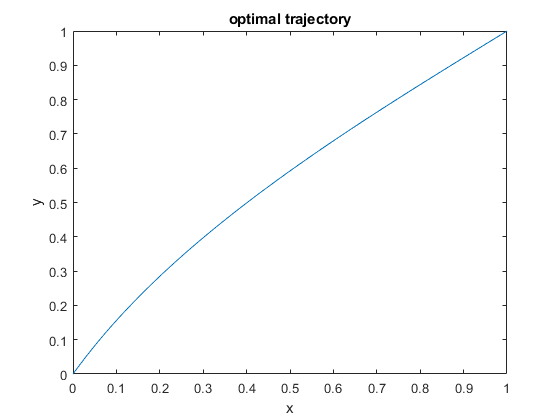
\includegraphics[width=0.5\textwidth]{./figures/5.2b.png}
	\caption{See the end of homework for code.}
\end{figure}
\end{enumerate}
\end{problem}
\begin{problem}[3]
The Hamiltonian is
 \begin{align*}
	H = u +p(- \alpha x+u) = (p+1)u - \alpha p x
\end{align*}
So the switching function is $ p+1$. Since the Hamiltonian is linear in $ u$, we want to use the Pontryagin maximum principle. To minimize $ H(x^* ,u,p^* ,t)$, we want to make  $ (p+1)u$ as negative as possible. Thus
 \begin{align*}
	u^* = \begin{cases}
		m & p^* <-1\\
		0& p^* >-1
	\end{cases}
\end{align*}
I claim that $ p^*  \neq -1$. Suppose $ p^* =1$. Since $ T$ is free, transversality yields  $ H(T) = 0$. But since  $ H$ is time-independent,  $ H$ is constant so  $ H \equiv 0$. However, we see that
 \begin{align*}
	H(0) = 0 \cdot u - \alpha (-1) x(0) = \alpha a >0,
\end{align*}
a contradiciton.

Now solving $ \dot{p} = -H_x = \alpha p$, we get $ p(t) = K e^{ \alpha p$. Notice that this is a monotone function and therefore can at most cross the line $ p=-1$ once. That is, the control will switch at most once.
\begin{case}[1]
If $ K \geq 0$,  $ p(t) > -1$ for all  $ t$ so we have no switching and  $ u^* =0$. Then solving $ \dot{x} = - \alpha x $ yields $ x(t) = K_1 e^{- \alpha t}$ and $ x(0) = K_1 = a$. Moreover, we have
\begin{align*}
	x(T) = a e^{- \alpha T} &= c \\
	e^{- \alpha T} &= \frac{c}{a} >0 \\
	- \alpha T &= \ln \frac{c}{a} \\
	T &=  \frac{1}{ \alpha} \ln \frac{a}{c} 
\end{align*}
If $ a>c$, then  $ \frac{a}{c}>1$ and $ T >0$. Thus, $J^* = 0 $. But if $ a\leq c$, then  $ T \leq 0$ which is unphysical. Thus in the case when $ K \geq 0$, $ a>c$, we have $ u^* \equiv 0$.
\end{case}
\begin{case}[2]
If $ K < 0$,  $ p$ might cross the line  $ p=-1$ once from above. Since $ p(0) = K$ starts in the $ p>-1$ regime, we have $ u^*(0) = 0$. But
\begin{align*}
	H(0) = (p(0)+1) u(0) - \alpha p(0) x(0) &= 0 \\
	- \alpha a p(0) &= 0 \\
	K=p(0) &= 0 && \alpha, a>0,
\end{align*}
a contradiction. Thus in this case we also have no switching and $ u^*  \equiv m$. Then we solve
\begin{align*}
	\dot{x} &= - \alpha x+m \\
\frac{dx}{m- \alpha x} &=  dt \\
x(t) &= \frac{m}{ \alpha} - K_2 e^{- \alpha t} \\
x(0) &= \frac{m}{ \alpha} - K_2 = a \\
x(t) &=  \frac{m}{ \alpha} - \left( \frac{m}{ \alpha}-a \right) e^{- \alpha t}  
\end{align*}
We have
\begin{align*}
	x(T) = \frac{m}{ \alpha} - \left(  \frac{m}{ \alpha} - a \right) e^{- \alpha T} &= c \\
	T &=  \frac{1}{ \alpha} \ln \left( \frac{m- \alpha a}{m- \alpha c } \right)  
\end{align*}
If $ a<c$, we see that  $ T>0$, and  $ J^*  = m T = \frac{m}{ \alpha} \ln \left( \frac{m- \alpha a}{ m- \alpha c} \right) $. If $ a \geq c$, we get  $ T \leq 0$ which is unphysical. Thus in the case when  $ K<0$,  $ a<c$, we have  $ u^*  \equiv m$.
\end{case}
\end{problem}

\begin{problem}[4]
\begin{enumerate}[label=(\alph*)]
\item We obtain
	\begin{align*}
		\begin{cases}
			\dot{x} = 15 \cos \theta +2\\
			\dot{y} = 15 \sin \theta -6
		\end{cases}
	\end{align*}
	So the Hamiltonian is
	\begin{align*}
		H=1+p_1(15 \cos \theta + 2) + p_2 (15 \sin \theta -6) .
	\end{align*}
	Adjoint equations yields that $ p_1$ and $ p_2$ are constants. First-order condition yields
	\begin{align*}
		H_{ \theta} = -15 p_1 \sin \theta + 15 p_2 \cos \theta &= 0 \\
		\tan \theta &= \frac{p_2}{ p_1} 
	\end{align*}
so $ \theta$ is also constant. We can integrate to get
\begin{align*}
	x(t) &= (15 \cos \theta+2) t -20\\
	y(t) &= (15 \sin \theta - 6) t  
\end{align*}
Using the terminal conditions, we solve
\begin{align*}
	\begin{cases}
		(15\cos \theta +2 )t_f -20 = -15 \\ 
		(15 \sin \theta -6)t_f = 35.5 
	\end{cases}
\end{align*}
which yields $ \theta^*  = 1.6198$ and $ t_f = 3.9524$. Since $ t_f$ is free, transversality condition yields
	 \begin{align*}
		H(t_f) =0
	\end{align*}
Since everything in $ H$ is a constant, $ H$ is a constant and must equal to $0$.
~\begin{figure}[H]
	\centering
	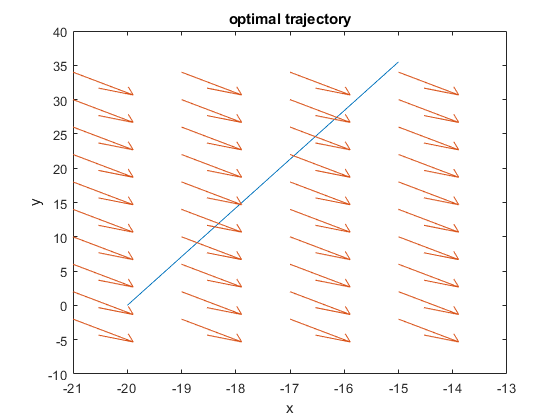
\includegraphics[width=0.5\textwidth]{./figures/5.4a.png}
	\caption{The optimal trajectory is a straight line.}
\end{figure}
\item The only thing changed here is the transversality conditions:
\begin{align*}
	H(t_f) &= \psi_t \lambda = 0 \\
	-p_1(t_f)  &= \psi_x \lambda =\lambda(-0.25-0.006 x_f^2) \\
	-p_2(t_f) &= \psi_y \lambda = -\lambda 
\end{align*}
where $ \psi(x_f,y_f)$ is the terminal constraint. Thus
 \begin{align*}
	\tan \theta = \frac{p_2}{ p_1} = \frac{1}{0.25+0.006 x_f^2}
\end{align*}
is still constant. This allows us to integrate the dynamics with the same initial conditions just as part (a).
\begin{align*}
	x(t) &= (15 \cos \theta+2) t -20\\
	y(t) &= (15 \sin \theta - 6) t  
\end{align*}
Now we can use the equations above to obtain $ x_f$ and  $ y_f$ in terms of  $ \theta$ and $ t_f$, and plug them into the terminal constraint and first-order condition:
 \begin{align*}
\begin{cases}
	25-0.25x_f - 0.002x_f^3-y_f = 0 \\
\tan \theta = \frac{1}{0.25+0.006x_f^2} 
\end{cases}
\end{align*}
and obtain $ \theta^*  = 1.3031 $, $ t_f =3.0144$, which yields $ x_f=-2.0114$ and  $ y_f = 25.5191$. Similar to part (a), the Hamiltonian consists of only constants so it is constant (zero).
~\begin{figure}[H]
	\centering
	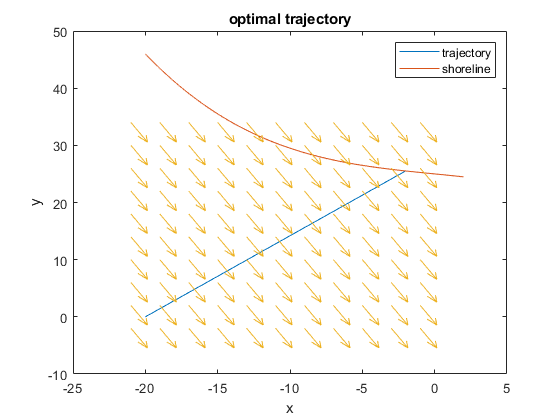
\includegraphics[width=0.5\textwidth]{./figures/5.4b.png}
	\caption{The optimal trajectory is still a straight line.}
\end{figure}
\item The dynamics becomes
\begin{align*}
	\begin{cases}
		\dot{x} = 15 \cos \theta -(y-50)\\
		\dot{y} = 15 \sin \theta + 2(x-15)
	\end{cases}
\end{align*}
And the Hamiltonian becomes
\begin{align*}
	H = 1+ p_1 (15 \cos \theta - (y-50)) + p_2(15 \sin \theta + 2(x-15))
\end{align*}
The adjoint equations become
\begin{align*}
	\dot{p}_1 &= -H_x = -2p_2 \\
	\dot{p_2} &= -H_y = p_1
\end{align*}
that satisfying the same transversality conditions as part (b). We still have
\begin{align*}
	\tan \theta = \frac{p_2}{ p_1}
\end{align*}
from first-order condition, although it is no longer constant. Moreover,
\begin{align*}
	\frac{d}{dt} H_{ \theta} &= -15 \dot{p}_1 \sin \theta - 15 p_1 \cos \theta \dot{\theta} + 15 \dot{p}_2 \cos \theta -15 p_2 \sin \theta \dot{\theta} =0\\
	2p_2 \sin \theta + p_1 \cos \theta &= (p_1 \cos \theta + p_2 \sin \theta) \dot{\theta}\\
	\dot{\theta} &=1+ \frac{p_2 \sin \theta}{ p_1 \cos \theta + p_2 \sin \theta } = 1+ \frac{1}{\cot^2\theta+1} = 1+ \sin^2\theta
\end{align*}
with boundary condition
 \begin{align*}
	\tan \theta(t_f) = \frac{p_2(t_f)}{p_1(t_f) } =\frac{1}{0.25+0.006x_f^2}
\end{align*}
Together with state dynamics, initial conditions, and the terminal constraint, we obtain the following solution with $ t_f = 0.8974$:
~\begin{figure}[H]
	\centering
	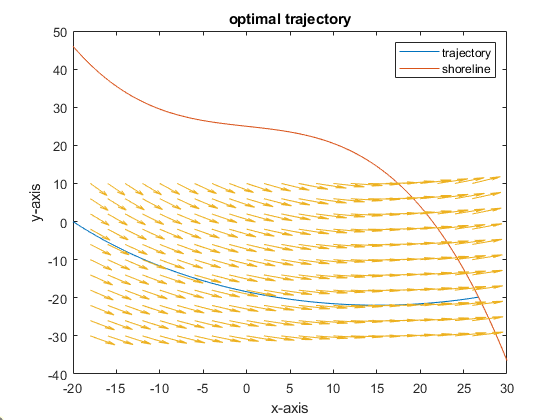
\includegraphics[width=0.5\textwidth]{./figures/5.4c.1.png}
	\caption{The trajectory aligns closely with the current this time.}
	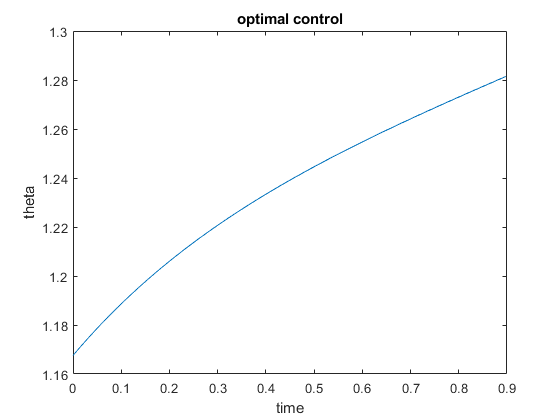
\includegraphics[width=0.5\textwidth]{./figures/5.4c.2.png}
	\caption{The optimal control $ \theta$.}
\end{figure}
We can compute the Hamiltonian by solving for $ p_1,p_2$ and $ \lambda$ using three transversality conditions of $ p_1(t_f),p_2(t_f)$, and $ H(t_f) =0$, but I ran out of time to do it.

\end{enumerate}
\end{problem}

\begin{problem}[5]
\begin{enumerate}[label=(\alph*)]
\item We have $ J = \max x(t_f) = - \min - x(t_f)$ so $ \phi(x_f)=-x_f$ and
\begin{align*}
	\begin{cases}
		\dot{x} = \cos \theta + u_0 \sin^2y\\
		\dot{y} = \sin \theta\\
	\end{cases}
\end{align*}
The Hamiltonian is
\begin{align*}
	H = p_1(\cos \theta + u_0 \sin^2 y) + p_2 \sin \theta
\end{align*}
The adjoint equations yield $ p_1$ is constant,
\begin{align*}
	 \dot{p_2} = -p_1 u_0 \sin 2y
\end{align*}
Since $ x(t_f)$ is free, transversality condition yields
 \begin{align*}
	p_1 \equiv p_1(t_f) = \phi_{x_f} = -1
\end{align*}
First-order condition yields
\begin{align*}
	H_{ \theta} = -p_1 \sin \theta + p_2 \cos \theta=\sin \theta+p_2 \cos \theta &= 0 \\
	\tan \theta = -p_2
\end{align*}
Hence we solve the following system:
\begin{align*}
	\begin{cases}
		\dot{x} = \frac{1}{ \sqrt{1+p_2^2} } + u_0 \sin^2 y\\
		\dot{y} = -\frac{p_2}{ \sqrt{1+p_2^2} }\\
		\dot{p_2} = u_0 \sin 2y
	\end{cases}
\end{align*}
with $ x(0) = y(0)=0$ and  $ y(t_f) = 0$.
\item We solve the Ricatti equation to find the conjugate point (when $ P$ blows up). We have  $ R_2 = H_{ \theta \theta} = \cos \theta - p_2 \sin \theta$, $ R_{12} = H_{xu} = 0$, and $ R_1 = \begin{pmatrix} 0&0\\0&-2u_0 \end{pmatrix} $. Furthermore, $ A(t) = \frac{\partial f}{\partial x} = \begin{pmatrix} 0&u_0 \sin 2y\\0&0 \end{pmatrix} $ and $ B(t) = \frac{\partial f}{\partial \theta} = \begin{pmatrix} -\sin \theta\\cos \theta \end{pmatrix} $. Staying on $ x$-axis means that  $ \theta =0$ and $ y=0$ throughout, so we have the following (with $ R_2 =1>0$ so regular):
 \begin{align*}
	 \widetilde{ A} &= A - BR_2^{-1}R_{12}^{T} = 0 -0=0\\
	 \Sigma &=  BR_2^{-1} B = \begin{pmatrix} 0\\1 \end{pmatrix} 1 \begin{pmatrix} 0&1 \end{pmatrix} = \begin{pmatrix} 0&0\\0&1 \end{pmatrix}  \\
	 \widetilde{ R} &= R_1 - R_{12}R_2^{-1}R_{12}^{T} = R_1 = \begin{pmatrix} 0&0\\0&-2u_0 \end{pmatrix}  
\end{align*}
Then Ricatti equation states:
\begin{align*}
	-\dot{P} &= 0+0- \begin{pmatrix} p_{11}&p_{12}\\p_{21}&p_{22} \end{pmatrix} \begin{pmatrix} 0&0\\0&1 \end{pmatrix} \begin{pmatrix} p_{11}&p_{12}\\p_{21}&p_{22} \end{pmatrix}  + \begin{pmatrix} 0&0\\0&-2u_0 \end{pmatrix} \\
	\begin{pmatrix} p_{11}&p_{12}\\p_{21}&p_{22} \end{pmatrix} &= \begin{pmatrix} p_{12}^2&p_{12}p_{22} \\p_{12}p_{22}&p_{22}^2+2u_0 \end{pmatrix}  \\ 
	\dot{p_{22}} &= p_{22}^2+2u_0\\
	p_{22}(t) &= \sqrt{2u_0} \tan \left( \sqrt{2u_0} (t-t_f) \right)   && P(t_f) =0
\end{align*}
We know that $ \tan t$ blows up at $ t = \frac{\pi}{ 2}+k \pi, k \in \zz$. Thus $ p_{22}$ blows up at
\begin{align*}
	t_k = \frac{1}{\sqrt{2u_0} } \left( \frac{\pi}{ 2}+k\pi \right) + t_f
\end{align*}
The conjugate point $ t_c$ is the first singularity encountered since the starting time $ t=0$. Thus  $ t_c$ has the smallest $k $ s.t.\ $ t_c >0$. Thus  $ x$-axis is a maximizing path only when there is no conjugate point,  \emph{i.e.} $ t_f<t_c$.
\end{enumerate}
\end{problem}
\begin{lstlisting}
%%%%%%%%%%%%%%%%%%%%%%%%%%%%%%%%%%%%%%%%%%%%%%%%%%%%%%%%%%%%%%%%%%%%%%%%%%
%Problem 2(b)
solinit=bvpinit(linspace(0,1),[1,1,-2.2],1.2); %tau is in [0,1]
sol2=bvp4c(@odehw52,@bchw52,solinit);

x=sol2.y(1,:);
y=sol2.y(2,:);
theta = sol2.y(3,:);
tf= sol2.parameters;
time=tf*sol2.x;

figure
plot(x,y)
xlabel('x');
ylabel('y');
title('optimal trajectory');

function dydt = odehw52(t,y,tf)
dydt = tf*[cos(y(3))-0.2*(3*y(2)-y(2)^3)
           sin(y(3))
           0.6*(1-y(2)^2)*cos(y(3))^2];
end

function res = bchw52(ya,yb,tf)
res = [ya(1)-1
       yb(1)
       ya(2)-1 
       yb(2)];
end

%Problem 4(a)
syms theta t
eqn=[(15*cos(theta)+2)*t-20==-15,(15*sin(theta)-6)*t==35.5];
sol4a=solve(eqn);

tf=double(sol4a.t);
tf=tf(1); %choose positive solution
theta = double(sol4a.theta);
theta = theta(1);

time=linspace(0,tf);
x=(15*cos(theta)+2)*time-20;
y=(15*sin(theta)-6)*time;
figure
plot(x,y)
hold on

[X, Y] = meshgrid(-21:2:-14, -2:4:36);
u = 2*ones(size(X));
v = -6*ones(size(Y));

% Normalize vectors for better visualization
magnitude = sqrt(u.^2 + v.^2);
u = u ./ magnitude;
v = v ./ magnitude;

quiver(X, Y, u, v);
hold off
xlabel('x');
ylabel('y');
title('optimal trajectory');

%Problem 4(b)
syms tf theta
x=@(t) (15*cos(theta)+2)*t-20;
y=@(t) (15*sin(theta)-6)*t;
eqn=[theta==atan(1/(0.25+0.006*x(tf)^2)),25-0.25*x(tf) ...
    -0.002*x(tf)^3-y(tf)==0];
sol4b = solve(eqn);
theta4b = double(sol4b.theta);
tf4b = double(sol4b.tf);

x=@(t) (15*cos(theta4b)+2)*t-20;
y=@(t) (15*sin(theta4b)-6)*t;
xf4b = x(tf4b);
yf4b = y(tf4b);

f=@(x) 25-0.25*x-0.002*x.^3; 
xplot = linspace(-20,2);

[X, Y] = meshgrid(-21:2:0, -2:4:36);
u = 2*ones(size(X));
v = -6*ones(size(Y));
% Normalize vectors for better visualization
magnitude = sqrt(u.^2 + v.^2);
u = u ./ magnitude;
v = v ./ magnitude;
time=linspace(0,tf4b);

figure
plot(x(time),y(time))
xlabel('x');
ylabel('y');
title('optimal trajectory');
hold on
plot(xplot,f(xplot))
quiver(X, Y, u, v);
hold off
legend('trajectory','shoreline')

%Problem 4(c)
tinit = linspace(0,1);
solinit=bvpinit(tinit,@guess54,3); %tau is in [0,1]
sol4c=bvp4c(@odehw54,@bchw54,solinit);

x=sol4c.y(1,:);
y=sol4c.y(2,:);
theta = atan(sol4c.y(3,:));
tf= sol4c.parameters;
time=tf*sol4c.x;
f=@(x) 25-0.25*x-0.002*x.^3; 
xplot = linspace(-20,30);

[X, Y] = meshgrid(-18:2:26, -30:4:10);
u = -(Y-50);
v = 2*(X-15);
% Normalize vectors for better visualization
magnitude = sqrt(u.^2 + v.^2);
u = u ./ magnitude;
v = v ./ magnitude;

figure
plot(x,y)
xlabel('x');
ylabel('y');
title('optimal trajectory');
hold on
plot(xplot,f(xplot))
quiver(X, Y, u, v);
hold off
legend('trajectory','shoreline')

figure
plot(time,theta)
xlabel('time');
ylabel('theta');
title('optimal control');

function dydt = odehw54(t,y,tf)
dydt = tf*[15*cos(y(3))-y(2)+50 %x
           15*sin(y(3))+2*(y(1)-15) %y
           1+sin(y(3))^2]; %theta
end

function res = bchw54(ya,yb,tf)
res = [ya(1)+20 %x0
       ya(2) %y0
       25-0.25*yb(1)-0.002*yb(1)^3-yb(2) %endpoint constraint
       tan(yb(3))-1/(0.25+0.006*yb(1)^2)]; %transversality costates
end

function g=guess54(t)
xinit = @(t) -20+t;
yinit = @(t) -t;
g=[xinit(t) yinit(t) 1];
end

%Problem 5

syms p22(t) u0 tf
sol5=dsolve(diff(p22,t)==2*u0+p22^2,p22(tf)==0);
%%%%%%%%%%%%%%%%%%%%%%%%%%%%%%%%%%%%%%%%%%%%%%%%%%%%%%%%%%%%%%%%%%%%%%%%%%
\end{lstlisting}
\end{document}
